% !TeX root = ..\main.tex

%%%%%%%%%%%%%%%%%%%%%%%%%
\section{Giới thiệu đề tài}

\hspace{0.5cm}Quy trình nghiệp vụ là một chuỗi các hành động diễn ra có thứ tự để cùng nhau hoàn thành một mục tiêu hoặc đạt được mục đích đề ra. Quy trình nghiệp vụ là một thành phần quan trọng trong quá trình hoạt động của một doanh nghiệp, chúng đại diện cho một trong những tài sản cốt lõi của các tổ chức. Chúng có tác động trực tiếp đến sức hấp dẫn của sản phẩm và dịch vụ, ảnh hưởng đến trải nghiệm của khách hàng và cuối cùng là ảnh hưởng đến doanh thu của doanh nghiệp. Các quy trình nghiệp vụ phối hợp cùng nhau để đáp ứng các nhu cầu từ người dùng, do đó các quy trình này cần được thiết kế đúng với nhu cầu của người dùng và hệ thống. Cụ thể, quy trình nghiệp vụ xác định các công việc và trách nhiệm của mỗi thành phần trong doanh nghiệp, thứ tự thực thi của các thành phần và hướng xử lý khi có lỗi. Các quy trình nghiệp vụ là hệ thống quan trọng trong tổ chức và trong mạng lưới cung ứng liên tổ chức. Do đó, bất kỳ lỗi quy trình nào cũng có thể khiến hoạt động của công ty và toàn bộ hệ sinh thái bị đình trệ.\\

Quy trình nghiệp vụ có tầm quan trọng là vậy, tuy nhiên quản lý việc vận hành quy trình nghiệp vụ là một bài toán không hề dễ dàng. Với việc các doanh nghiệp ngày càng mở rộng quy mô kinh doanh, cùng sự tăng lên của tập người dùng, các quy trình nghiệp vụ cũng dần lớn lên, và thường phải thay đổi theo sự thay đổi của người dùng và thị trường. Sự thay đổi nhanh của các quy trình nghiệp vụ đòi hỏi một phương pháp quản lý hiệu quả hơn cho các quy trình này. Xuất phát từ nhu cầu đó, một bộ công cụ, kỹ thuật và phương pháp được sinh ra để hỗ trợ quản lý vòng đời quy trình nghiệp vụ đã xuất hiện và được sử dụng trong hai thập kỷ qua. Nó được gọi là \textbf{Quản lý quy trình nghiệp vụ (BPM)}. BPM được tin dùng cho nhiều lĩnh vực khác nhau, bao gồm kỹ thuật công nghiệp, quản lý hoạt động, quản lý chất lượng, quản lý nguồn nhân lực, quản trị doanh nghiệp, khoa học máy tính và kỹ thuật, hệ thống thông tin.\\

Trong quá trình thực thi quy trình nghiệp vụ, những quy trình có thể cần được cải thiện và thay đổi. Khi sửa đổi quy trình, doanh nghiệp cần đảm bảo chương trình chạy đúng như quy trình mới. Việc thay đổi mã nguồn bằng tay để thay đổi luồng thực thi chương trình sẽ tiêu tốn rất nhiều thời gian và công sức; tuy vậy, sai lầm lại rất dễ xảy ra. Từ đây, nhu cầu áp dụng công nghệ vào việc tự động hóa các quy trình được đặt ra. Để đáp ứng nhu cầu này, phương pháp \textbf{Tự động hóa quy trình nghiệp vụ (BPA)} được ra đời. Thay vì dùng con người, phương pháp này sử dụng công nghệ và phần mềm để tự động hóa các quy trình nghiệp vụ. Trái ngược với các loại tự động hóa khác, các giải pháp BPA có xu hướng phức tạp, được kết nối với nhiều hệ thống công nghệ thông tin  và được điều chỉnh cụ thể theo nhu cầu của một tổ chức. Các tổ chức thường áp dụng BPA như một phần của chiến lược chuyển đổi kỹ thuật số, nhằm hợp lý hóa quy trình nghiệp vụ của mình và đảm bảo hiệu quả hoạt động. Tự động hóa quy trình nghiệp vụ có thể giải phóng thời gian và nguồn lực cho doanh nghiệp rất nhiều.\\

Với các yêu cầu về thiết kế và quản lý quy trình nghiệp vụ như trên, Lược đồ mô hình hóa quy trình nghiệp vụ (BPMN) là một lựa chọn rất hữu ích. Đây là ngôn ngữ hướng đồ thị, cung cấp cho doanh nghiệp khả năng thiết kế các quy trình nghiệp vụ của mình dưới dạng lược đồ, đồng thời đặt ra tiêu chuẩn chung cho các doanh nghiệp truyền đạt các quy trình nghiệp vụ. Việc biểu diễn các quy trình nghiệp vụ theo dạng lược đồ giúp cho doanh nghiệp quản lý tốt hơn hoạt động kinh doanh của mình khi mọi phòng ban đều có thể hiểu ngôn ngữ ở dạng lược đồ. Để thực thi quy trình nghiệp vụ được thiết kể bởi BPMN, chúng ta cần sử dụng đến Ngôn ngữ thực thi quy trình nghiệp vụ (BPEL). BPMN đóng vai trò phác thảo các quy trình nghiệp vụ, là công cụ để các thành phần trong doanh nghiệp có thể trao đổi và thiết kế quy trình nghiệp vụ. Sau khi thiết kế BPMN, BPEL là ngôn ngữ để vận hành các quy trình nghiệp vụ đó. Với BPMN và BPEL, ta có thể dễ dàng tự động hóa quy trình nghiệp vụ, bảo đảm quy trình nghiệp vụ được vận hành chính xác, và việc cập nhật quy trình nghiệp vụ sẽ được đáp ứng vào hệ thống dễ dàng.\\

Bằng cách sử dụng các công cụ và công nghệ đã trình bày ở trên, nhóm sẽ thực hiện tự động hóa quy trình nghiệp vụ doanh nghiệp, và áp dụng vào một hệ thống cửa hàng thời trang trong đề tài: "Xây dựng ứng dụng quản lý hệ thống cửa hàng thời trang dựa trên việc tự động hóa quy trình nghiệp vụ".
%%%%%%%%%%%%%%%%%%%%%%%%%

\section{Mục tiêu đề tài}
\hspace{0.5cm}Mục tiêu của đề tài là nghiên cứu và áp dụng tự động hóa quy trình nghiệp vụ vào trong một hệ thống cửa hàng thời trang. Việc vận hành hệ thống cần đảm bảo các yêu cầu chức năng và phi chức năng, đồng thời bao gồm các tính năng đã đề ra. Về phần quy trình nghiệp vụ, nghiệp vụ của hệ thống được quản lý và tự động hóa bằng phương pháp tự động hóa quy trình nghiệp vụ. Việc thiết kế và cập nhật nghiệp vụ sẽ được diễn ra nhanh chóng, dễ dàng dưới sự trợ giúp của BPMN và BPEL.

%%%%%%%%%%%%%%%%%%%%%%%%%
\section{Phạm vi đề tài}
\hspace{0.5cm}Trong đề tài này, nhóm sẽ áp dụng BPMN để thiết kế các quy trình nghiệp vụ cho một hệ thống cửa hàng thời trang, và sử dụng BPEL để thực thi quy trình nghiệp vụ. Nhóm sẽ phân tích, thiết kế và hiện thực một hệ thống bán hàng thời trang, bao gồm các tính năng mua / bán hàng trực tuyến và trực tiếp, và các tính năng quản lý hoạt động của hệ thống bán hàng.

%%%%%%%%%%%%%%%%%%%%%%%%%
\section{Ý nghĩa đề tài}
\hspace{0.5cm} Trong thực tế, quy trình nghiệp vụ của doanh nghiệp thường lớn và phức tạp, đòi hỏi sự tham gia của nhiều thành phần có các mối liên hệ phức tạp với nhau. Một sự thay đổi nghiệp vụ đòi hỏi nhiều thời gian và công sức để áp dụng vào hệ thống thực tế. Đối với phần lập trình và phát triển hệ thống, lập trình viên cần thay đổi mã nguồn ở nhiều nơi để đáp ứng đúng với thay đổi của nghiệp vụ, và cần đảm bảo sau khi thay đổi hệ thống vừa chạy đúng với nghiệp vụ mới, vừa đáp ứng các yêu cầu chức năng và phi chức năng đã đặt ra từ đầu. Với cách tiếp cận này, việc thay đổi và cập nhật quy trình nghiệp vụ sẽ tốn nhiều thời gian khi phải thay đổi mã nguồn ở nhiều phần trong hệ thống, sẽ tốn công sức để đảm bảo hệ thống đáp ứng đúng như yêu cầu sau cập nhật, và dễ có rủi ro nếu việc tìm và thay đổi mã nguồn vẫn chưa triệt để.\\

Với sự giúp đỡ của việc tự động hóa quy trình nghiệp vụ, việc quản lý quy trình nghiệp vụ sẽ trở nên dễ dàng hơn rất nhiều. Quy trình nghiệp vụ có thể được biểu diễn dưới dạng mô hình BPMN - một mô hình có thể hiểu được bởi người dùng nghiệp vụ và lập trình viên. Việc thay đổi và cập nhật quy trình nghiệp vụ sẽ được tối ưu và tự động với Ngôn ngữ thực thi quy trình nghiệp vụ - BPEL. Các thành phần của hệ thống tương ứng với các bước trong quy trình nghiệp vụ sẽ được kết nối đến các thành phần của BPEL, do đó khi có sự thay đổi của quy trình nghiệp vụ, chỉ cần cập nhật lại BPEL thì BPEL sẽ gọi thứ tự thực thi nghiệp vụ mới theo đúng như nó được cập nhật. Do đó, lập trình viên không cần tìm và sửa mã ở khắp nơi trong mã nguồn, mà chỉ cần cập nhật BPEL và đảm bảo kết nối đúng các thành phần BPEL đến các thành phần trong hệ thống. Do BPEL là một ngôn ngữ thực thi, nó có thể được deploy và chạy, nên khi có sự thay đổi nghiệp vụ ở BPMN và BPEL, việc cập nhật nghiệp vụ sẽ nhanh và tự động mà không yêu cầu nhiều công sức của con người.

%%%%%%%%%%%%%%%%%%%%%%%%%
\section{Đóng góp của đề tài}
\hspace{0.5cm} Đề tài mong muốn chứng minh sự hiệu quả khi áp dụng BPMN và BPEL vào việc thiết kế và quản lý quy trình trong mỗi doanh nghiệp. Sau khi hoàn thành, đề tài muốn cho thấy cách tiếp cận bằng tự động hóa quy trình nghiệp vụ sẽ giảm đáng kể thời gian và nguồn lực trong việc quản lý quy trình nghiệp vụ, và sẽ mang lại hiệu quả lớn cho doanh nghiệp trong việc vận hành hệ thống của mình.

%%%%%%%%%%%%%%%%%%%%%%%%%   
\section{Phân chia công việc}
 {


  \begin{figure}[h]
	  \begin{center}
		  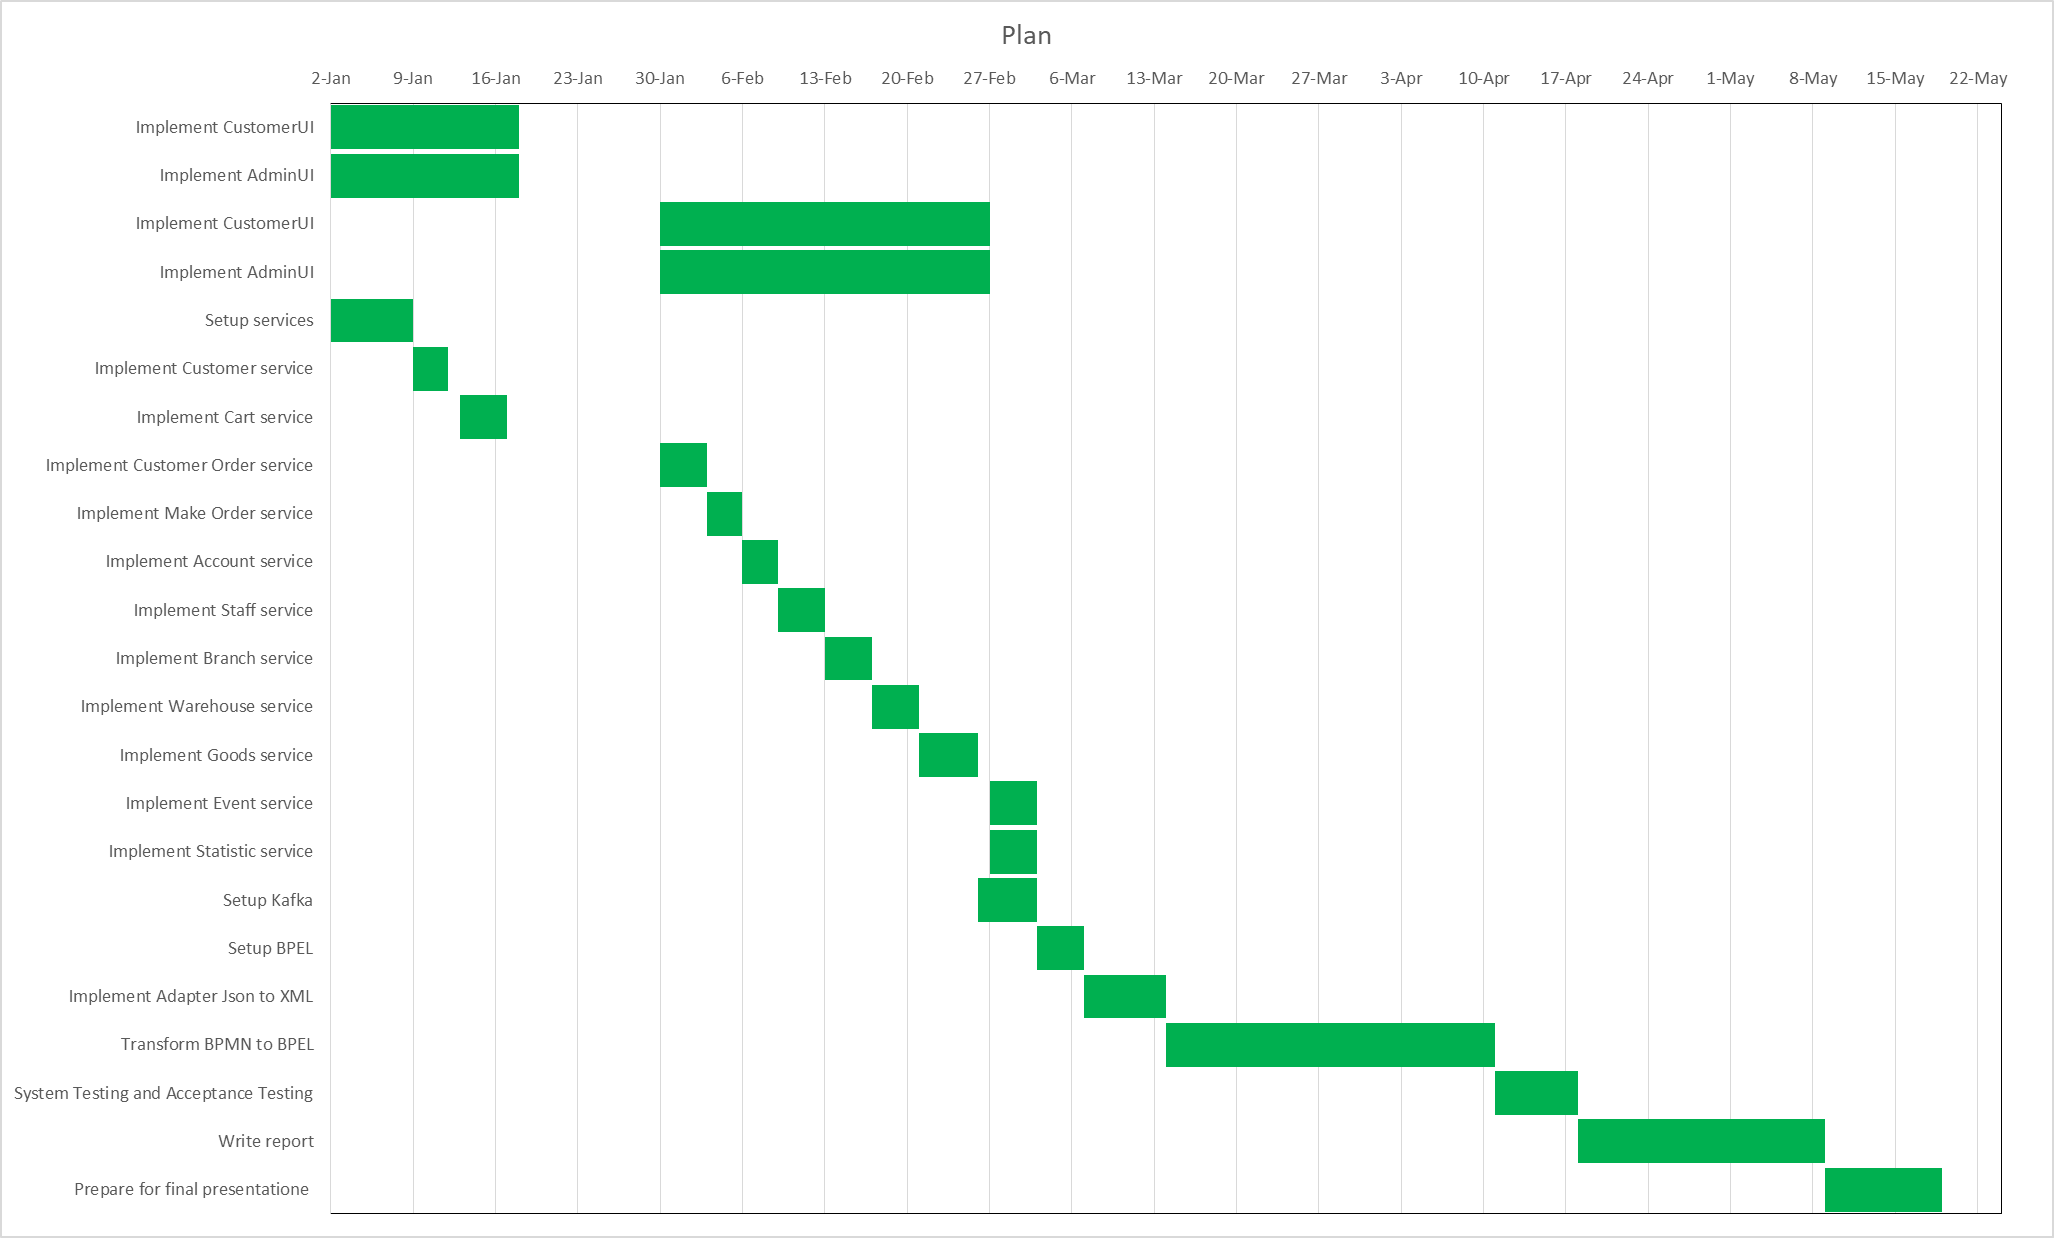
\includegraphics[width=14cm]{img/plan.png}
	  \end{center}
	  \caption{Biểu đồ Gantt quá trình thực hiện đồ án tốt nghiệp}
  \end{figure}


  \newpage

  \setlength\extrarowheight{6pt}
  \begin{longtable}{| p{2cm} | p{2cm} | p{10cm} |}

	  \hline
	  \textbf{Bắt đầu} & \textbf{Hạn} & \textbf{Công việc}                                             \\
	  \hline
	  02/01/2023       & 08/01/2022   &
	  - Phong: Setup môi trường cho CustomerUI và hiện thực layout.
	  \newline
	  - Hiển: Setup môi trường cho AdminUI và hiện thực layout.
	  \newline
	  - Thọ: Setup môi trường cho backend, khởi tạo các service và đảm bảo giao tiếp giữa các service. \\
	  \hline
	  09/01/2023       & 16/09/2022   &
	  - Phong: Hiện thực Login page - Register page và Reset Password page.
	  \newline
	  - Hiển: Hiện thực Branch page - Branch detail page - Order page - Order detail page.
	  \newline
	  - Thọ: Hiện thực Customer service                                                                \\
	  \hline
	  30/01/2023       & 05/02/2022   &
	  - Phong: Hiện thực Home page - List Product page.
	  \newline
	  - Hiển: Hiện thực Event page - Event detail page - Goods page - Goods detail page, Goods Edit page.
	  \newline
	  - Thọ: Hiện thực Cart service.                                                                   \\
	  \hline
	  06/02/2023       & 12/02/2022   &
	  - Phong: Hiện thực Product Detail page - Cart page.
	  \newline
	  - Hiển: Hiện thực Staff page - Staff Detail page - Staff Request page.
	  \newline
	  - Thọ: Hiện thực Order service                                                                   \\
	  \hline
	  13/02/2023       & 19/02/2022   &
	  - Phong: Hiện thực Payment page - Manager Order page.
	  \newline
	  - Hiển: Hiện thực Account page, Account Detail page.
	  \newline
	  - Thọ: Hiện thực Account service                                                                 \\
	  \hline
	  20/02/2023       & 26/02/2022   &
	  - Phong: Hiện thực Order Detail page và Customer Info page.
	  \newline
	  - Hiển: Hiện thực Warehouse page - Statistic page.
	  \newline
	  - Thọ: Hiện thực Staff service.                                                                  \\
	  \hline
	  27/02/2023       & 05/03/2022   &
	  - Phong: Refactor code cho CustomerUI, hiện thực Event service.
	  \newline
	  - Hiển: Refactor code cho AdminUI, hiện thực Statistic service.
	  \newline
	  - Thọ: Hiện thực Branch service.                                                                 \\
	  \hline
	  06/03/2023       & 12/03/2022   &
	  - Hiển           \& Phong: Nghiên cứu, chuyển đổi BPMN sang BPEL
	  \newline
	  - Thọ: Hiện thực Warehouse service.                                                              \\
	  \hline
	  13/03/2023       & 19/03/2022   &
	  - Hiển           \& Phong: Nghiên cứu, chuyển đổi BPMN sang BPEL
	  \newline
	  - Thọ: Hiện thực Goods service.                                                                  \\
	  \hline
	  20/03/2023       & 26/03/2022   &
	  - Hiển           \& Phong: Nghiên cứu, chuyển đổi BPMN sang BPEL
	  \newline
	  - Thọ: Hiện thực Event service.                                                                  \\
	  \hline
	  27/03/2023       & 02/04/2022   &
	  - Hiển           \& Phong: Nghiên cứu, chuyển đổi BPMN sang BPEL
	  \newline
	  - Thọ: Hiện thực Statistic service.
	  \newline
	  - Tất cả: Viết báo cáo                                                                           \\
	  \hline
	  03/04/2023       & 16/04/2022   &
	  - Hiển           \& Phong: Nghiên cứu, chuyển đổi BPMN sang BPEL.
	  \newline
	  - Thọ: Hiện thực BFF và các adapter
	  \newline
	  - Tất cả: Viết báo cáo                                                                           \\
	  \hline
	  17/04/2023       & 23/04/2022   &
	  - Hiển           \& Phong: Nghiên cứu, chuyển đổi BPMN sang BPEL.
	  \newline
	  - Thọ: Hiện thực kết nối Kafka
	  \newline
	  - Tất cả: Viết báo cáo                                                                           \\
	  \hline
	  24/04/2023       & 30/04/2022   &
	  - Tất cả thành viên: Tổng hợp hệ thống.
	  \newline
	  - Tất cả: Viết báo cáo                                                                           \\
	  \hline
	  01/05/2023       & 07/05/2022   &
	  - Hiển           \& Phong: Viết báo cáo và kiểm thử hệ thống
	  \newline
	  - Thọ: Triển khai hệ thống                                                                       \\
	  \hline
	  08/05/2023       & 14/05/2022   &
	  - Tất cả thành viên: Viết báo cáo, kiểm thử hệ thống                                             \\
	  \hline
	  15/05/2023       & 29/05/2022   &
	  - Tất cả thành viên: Chuẩn bị cho phản biện và bảo vệ đề tài                                     \\
	  \hline
  \end{longtable}

 }